%!TEX root = ../thesis.tex
%*******************************************************************************
%****************************** Second Chapter *********************************
%*******************************************************************************

\chapter{Memristive Devices}

\section[Introduction]{Introduction}

The initial primary focus of this thesis is on the characterisation of silicon-based memristors, which are the fundamental components of memristive systems. Since the discovery of the memristor and its importance to replicating synaptic activity had such a profound impact on the field of neuromorphic engineering, investigating additional nanoelectronic components and behaviours in this context will lead to new neuromorphic computing applications. \\

\noindent This chapter investigates a phenomenon known as the "current transient" that has yet to be deliberately applied to the demand of neuromorphic computing. The current transient phenomenon can be similarly represented by the current flowing through a defective capacitor in response to a step potential to produce rich dynamics, both growing and decreasing in conductance, and can be beneficial in a computational device. \\

\noindent This chapter begins by documenting and characterising the current transients based on available literature. The experimental procedures used throughout the chapter were then described, and strategies were developed to aid in the characterisation of current transients. This provides a deeper understanding of the physical models underpinning the transients, allowing for the further development of an integrative memristive system based on silicon oxide samples that are already available.

\subsection[Foundational Properties]{Foundational Properties}

Fundamentally, the processes of capacitive decay and dielectric relaxation are ideal to define a capacitor's response to a step voltage. Applying a constant voltage across its terminals causes the device current to decline until it ultimately comes to rest at a constant leakage current. This, however, is not always the case. When the voltage is applied for an extended period of time or at a high enough temperature, the current flowing through the device begins to grow as the oxide gets faulty and its resistance falls. This is known as oxide deterioration, an umbrella word for an oxide coating that becomes faulty over time as a result of environmental stress factors \cite{ghibaudo1999emerging}. \\

\noindent One specific form of this resistance degradation addressed here is the "current transient". This is distinguished by their characteristic form when plotted on a current-time graph as illustrated in Figure \ref{fig:2a}. When a voltage is applied to the device, the current grows swiftly to a maximum and then gradually decays, resulting in a distinctive peak in device current. Surprisingly, whereas oxide degradation is essentially a permanent impact, the change in oxide resistance that happens during a current transient is not; rather, it is volatile. \\

\begin{figure}[htbp!] 
\centering    
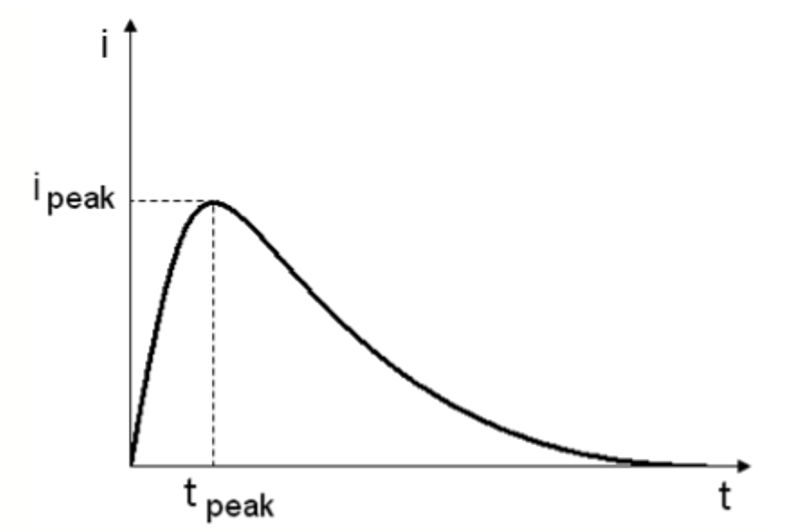
\includegraphics[width=0.5\textwidth]{Chapter3/Figs/3a.png}
\caption[Current transients illustration]{Current transient caused by a change in temperature for a closed circuit \cite{zafar2011measurement}, the plot is for illustration purpose only.}
\label{fig:3a}
\end{figure}

\noindent The most common differentiating feature is the combination of their distinct peak and their extended time periods during which they occur. Previously published papers documented peak periods ranging from 5 to 20 seconds, and the full transient is frequently seen for 10s to 100s of seconds \cite{saha2001transient}. They are both slow pace and long-lasting occurrences. Timescales of this magnitude are not usual for integrated resistor-capacitor (RC) circuits because they demand enormous capacitance, which necessitates physically much bigger capacitors \cite{el2006space}. \\

\noindent One appealing aspect of the phenomena is the much longer time periods of the current transient's responses in contrasted with a traditional RC circuit. However, the dynamics of the transient are not fixed. They are known to be accelerated by increases in applied temperature \cite{manceau2007metal}, voltage \cite{zafar1998oxygen}, and when irradiated with a laser \cite{li2015visible}. All of these variables can cause the transient to accelerate, with the peak coming sooner in time. When pushed far enough, the peak disappears completely and we only see a decreasing current, which is most likely owing to the instruments' temporal resolution. \\

\noindent Given that the features of transients have been similar across published research, it is worth noting that these studies have used a variety of oxide materials. However, despite being present in a variety of device setup, the current transient is not equally observed in every instance, and this is especially noticeable with regard to device polarity. Early investigations on current transients only detected transients in a single voltage polarity \cite{manceau2007current}, however other devices in the literature now produce transients in both polarities \cite{chen2010observation}. \\

\noindent Transients have been reported in a wide range of materials, implying that they are a generic phenomena that might occur in a wide range of MIM devices under the correct conditions. The current transient's characteristics deviate from the typical resistance switching behaviours reported in silicon oxide devices. They are analogous and volatile as compared to devices that display non-volatile binary switching when run in a normal resistance switching mode. Understanding the source and features of current transients is significant because they may have ramifications for a variety of research areas studying metal-oxide structures, such as transistor gates or the comparatively emerging subject of resistive switching memory.

\subsection[Current Models]{Current Models}
The most well-known model for explaining this behaviour is the Space Charge Limited Current (SCLC) hypothesis, which was created for describing a general space charge within a perfect insulator \cite{many1962theory}. A variety of theories have been offered up to describe this phenomenon \cite{lampert1970current}. Since charged oxygen vacancies are thought to constitute the space charge in question, this initial model was first associated with them. \\

\noindent Along with the electronic current, an ionic current also flows as a result of the drift of charged defects under an applied bias. The electrical contact at the other end blocks the charged defects, causing them to build up. The Coulombic repulsion that results from this buildup prevents further migration, which in turn reduces the ionic current as it starts to oppose itself. Because of this, earlier research assumed that the transient behaviours was caused by a general space charge inside of an insulator without any trapping in order to develop the SCLC model. \\

\noindent The original study only considered in one dimension and made the assumption that the conduction is planar. This might represent an ionic current or an electronic current, depending on whether the charges and mobilities correspond to electrons or some other charged defect inside the oxide. Recent study has assumed that the latter is the case. The mobility is frequently thought to refer to moving oxygen vacancies inside the oxide \cite{zafar1998oxygen}, or in other instances, to moving ions \cite{chen2010observation}; in all cases, it is supposed that the current is ionic. \\

\noindent Originally, the current of the model is defined as:
\begin{align}
j(t) &= j_{cond} + j_{disp} \label{eq:3.1} \\
j_{cond}(x,t) &= qn(x,t)\mu E(x,t) \label{eq:3.2} \\
j_{disp}(x,t) &= \epsilon \frac{\partial E(x,t)}{\partial t} \label{eq:3.3} \\
qn(x,t) &=  \epsilon \frac{\partial E(x,t)}{\partial x} \label{eq:3.4}
\end{align}

\noindent where $j(t)$ is the total current, $j_{cond}$ is the electronic conduction current, $j_{disp}$ is the displacement current, $q$ is the the charge of a single electron or the respective ion measured in Coulombs, $n$ is the space charge concentration, $\mu$ is the oxide space charge mobility, $E$ is the oxide local electric field, $L$ is the oxide thickness, $\epsilon$ is the oxide dielectric permittivity, $x$ is the position within the oxide ranging from 0 to $L$, $j$ is either the electronic or ionic current depending on the space charge, and lastly the Poisson's equation is denoted with equation \ref{eq:3.4}.
\begin{align}
j(t) &= \epsilon \left( \frac{\mu}{2} \frac{\partial E^{2}(x,t)}{\partial x} + \frac{\partial E(x,t)}{\partial x} \right) \label{eq:3.5} \\
j(t) &= \frac{\epsilon \mu}{2L}\left( E^{2}_{a}(t) - E^{2}_{c}(t) \right) \label{eq:3.6} \\
j(t) &= \frac{\mu Q(t)}{2L}\left( 2E_a(t) - \frac{Q(t)}{\epsilon} \right) \label{eq:3.7}
\end{align}

\noindent By substituting into the first equation, the device current density description can be derived to be (\ref{eq:3.5}). Assuming the voltage applied is fixed, the boundary conditions for the electric fields can be defined as $E_a(t) = E(L,t)$ and $E_c(t) = E(0,t)$ for the anode and the cathode respectively. Integrating (\ref{eq:3.5}) with respect to $x$ from the cathode to the anode yield equation \ref{eq:3.6} which describes the current as a function of the electric fields across the electrodes. \\

\noindent Note that the applied voltage was assumed to be non-varying with time, $\int_{0}^{L} \frac{\partial E(x,t)}{\partial t} dx = \frac{\partial }{\partial t} \int_{0}^{L}Edx = \frac{\partial V}{\partial t} = 0$, in a single dimension while the problem is intractable for spherical and cylindrical geometries \cite{lampert1970current}. This equation can further be rewritten with respect to the insulator total charge (\ref{eq:3.7}), with the relationship between the cathode and anode electric fields given as $E_a(t) = E_c(t) + \frac{q(t)}{\epsilon}$, where $Q(t)$ is the insulator total charge.
\begin{align}
\frac{E}{E_a^2} &= \frac{\mu}{2L} \partial t \label{eq:3.8} \\
E_a(t) &= \frac{V}{L}\left( 1 - \frac{\mu V}{2L^2} \right)^{-1} \label{eq:3.9}
\end{align}

\noindent After deriving an equation describing the device current, the subsequent step is to obtain the equation of the SCLC model that connects the mobility of the space charge with the time at which the peak $\tau$ appears. It is assumed that this is the instant when the charge front reaches the anode of the device. The derivation starts with the assumption that the field at the cathode is zero, $E_c(t) = 0$. \\

\noindent The next assumption is that the conduction component of the current is zero when evaluated at the anode of the device, $j_{cond} = 0$, as no charge has reached the anode yet, leaving $j(t)=\epsilon  \frac{\partial E(t)}{\partial t}$. This, combined with (\ref{eq:3.6}) and the prior assumption that the field is zero at the cathode, results in a differential equation having a solution as provided by equation \ref{eq:3.9}. 
\begin{align}
L &= \mu \int_{0}^{\tau} E_a(t) dt \label{eq:3.10} \\
L &= -2L \left[ ln \left( 1 - \frac{\mu V t}{2L^2} \right) \right]_0^{\tau} \label{eq:3.11} \\
\tau &= \frac{2 L^2}{\mu V} \left[ 1 - exp \left( -\frac{1}{2} \right) \right] \cong 0.787 \frac{L^2}{\mu V} \label{eq:3.12} 
\end{align}

\noindent After the field at the anode has been determined, it is now possible to calculate the time it takes for the front of the space charge to reach the anode. Assuming that the space charge's velocity is given by $\mu E(x,t)$, and the field is constant between the charge front and the anode, it can be assumed that the field experienced by the front of the space charge is equal to the field at the anode, $E(x,t) = E_a(t)$. \\

\noindent The time it takes for the charge front to cross the device can be determined by solving the integral (\ref{eq:3.10}), to get an analytical and approximated solution (\ref{eq:3.11}). This analysis has arrived at a significant equation of the SCLC model which has been widely used in the literature on current transients, frequently to determine the mobility of the space charge. To determine the equation's validity, it is necessary that the original model of the device's space charge traversing holds true. \\

% \noindent The prevalence of the SCLC model can be attributed to \ref{eq:2.12} and the appealing material properties it implies. For instance, it indicates the possibility of acquiring the mobility of the migrating defects that, when paired with the Einstein-Nernst equation, can disclose the activation energy of such defects. This equation has been used by researchers to determine the activation energies and mobility of different materials observed in current transients. According to some, the changes in the transient that occur due to laser illumination are evidence of accelerated mobility \cite{li2015visible} or charge transitions within the defect \cite{lee2019charge}. However, if researchers intend to use this model to derive mobilities and secondary observations based on changes in mobility, the model's validity must be ensured. This is where problems may arise.

\subsection[Additional Considerations]{Additional Considerations}

Naturally, SCLC is not the only model used to explain these transients. While SCLC argues that the transient is the outcome of a substantial ionic current, it could also be inferred that the ionic currents are insignificant, and the transient results from a variation in the electronic conductivity of the bulk and interfaces \cite{meyer2005oxygen}. This conclusion was reached by simulating the redistribution of vacancies, electrons, and holes within the BST oxide layer bounded by two Schottky contacts at the $BST-Pt$ interfaces. The simulation was conducted using a finite difference method, accounting for the redistribution of each particle species that is influenced by drift and diffusion. 
\begin{align}
    j_k = -D_k\frac{\mathrm{d} C_k}{\mathrm{d} x} + \frac{Z_k}{|Z_k|} \mu_k C_k E , \mbox{ where $k \in \left \{ n,p,V_{\ddot{o}} \right \}$ } \label{eq:3.13} 
\end{align}

\noindent The simulation iteratively establishes the particle redistribution and subsequently computes the total device current, which is based on the velocity and distribution of the particles. The total device current is composed of the electron, hole, and vacancy currents. For each particle species, the current comprises a diffusion and drift term, as outlined by the Nernst-Einstein equation \ref{eq:3.13}, where $k$ indicates particle species which can be electrons, holes or charged oxygen vacancies, $j_k$ is the current density, $D_k$ is the diffusion coefficient, $C_k$ is the particle concentration, $Z_k$ is the charge in Coulombs, $\mu_k$ is the mobility, and $E$ is the local electric field. This method is beneficial since it allows for separation of the electronic and ionic currents, which is not feasible in an experiment. \\

% \noindent Within the simulation, a rapid and asymmetric redistribution of electrons and holes is observed, resulting in a highly n-type interface at the negative electrode and the other slightly depleted from its resting electron concentration. Based on published data, this rate slows at the onset of the transient's peak. Following this redistribution of electrons is the migration of oxygen vacancies, which is a much slower process. Vacancies also migrate towards the negative electrode alongside the electrons. This strongly impacts the internal electric field, causing some bending of the conduction band. Due to the lower mobility of the vacancies and their slower migration, it is found that the corresponding ionic displacement current is too small to be the cause of the increase in device current. Instead, the increase is caused by the modulation in electronic conductivity due to the change in vacancy distribution.\\


\noindent By varying the temperature of the simulated device, it was determined that the activation energy for increased conductance is 0.8eV, which is deemed reasonable for vacancies within a BST device \cite{zhong2010transient}. However, as the peak of the transient has already taken place by the time the vacancies have redistributed to a considerable extent, it is advisable to refrain from asserting that the activation energy inferred from the peak characterises the migration of vacancies. \\

\noindent Instead, the published results suggest that this could be attributed to the migration of electrons and holes, which predominantly occurs prior to and during the peak. Other researchers have also reached a comparable conclusion \cite{zhong2010transient}. For instance, electronic traps were observed with apparent activation energies ranging from 0.18-0.3eV. It was concluded that oxygen vacancy migration results in alterations of electron/hole concentrations, ultimately regulating bulk conductivity. \\

\noindent With two conflicting theories in existence, certain studies aim to determine whether the effect is electronic or ionic (SCLC). For instance, transients in some devices were analysed by considering both the SCLC model and the modulation of electronic conductivity \cite{wakiya2006activation}. It was found that the model of electronic conductivity produces a more credible value for the dielectric constant, suggesting it is the superior model. \\

\noindent However, a different study \cite{el2006space} aimed to determine whether the effect is due to ionic or electronic currents by assuming that electronic traps would be influenced by the oxide's crystallinity. It was discovered that almost identical transients were observed in the amorphous and polycrystalline devices, suggesting that the effect is of an ionic nature, which is also further supported by a previous claim \cite{zafar1998oxygen}. \\

\noindent However, in a subsequent publication \cite{el2007ionic}, it was determined that an alternative theory, based on the existence of shallow electronic traps, also favoured an electronic explanation. It seems that the issue of whether this effect is ionic or electronic has not been definitively resolved. Nonetheless, the prevailing trend in the literature has been towards mostly electronic conduction, which is altered by the movement of vacancies.\\

\noindent Retrospectively, the SCLC model has been found to be helpful, but it has not yet been fully validated. It has been observed that higher temperatures and applied voltages cause an increase in the rate of the transient as predicted, and peak time plotted against reciprocal voltage has been found to be linear in certain regimes. However, the original space charge limited current (SCLC) model can enables us to provide more detailed scrutiny.\\

\noindent Take the thickness dependence of peak time, as stated in (\ref{eq:3.12}), as an example. This phenomenon results from vacancies traversing the oxide from one electrode to the other, and it should lead to the peak time being proportional to the square of the device thickness, $L$. Although no research has specifically investigated this issue, published data from a related study can be utilised to provide a preliminary assessment of this dependence.\\

% \noindent From previously published data \cite{manceau2007current}, it seems that the timing of the peak is not affected by the thickness of the device. The studies investigate three oxide thicknesses: 900\r{A}, 450\r{A} and 200\r{A}. An increase in peak time is anticipated. In comparison to the 200\r{A} device, the 450\r{A} device should have a peak timing 6 times greater, while the 900\r{A} device should have a peak timing 20 times greater. However, no such increase is observed, as the evidence demonstrates.\\

% \noindent Instead, it appears that the peak's height is affected, not its timing. In thinner samples, the peak appears more spread out, whereas in thicker samples, the peak is more pronounced. This disparity between the critical SCLC theory equation and experimental evidence raises concerns when applying this model, though it is not the sole concern.\\

\begin{figure}[htbp!] 
\centering    
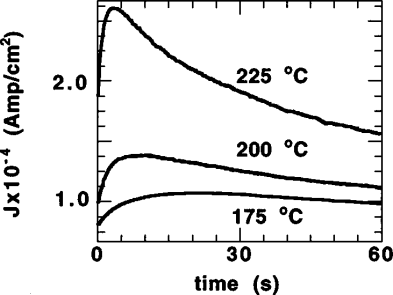
\includegraphics[width=0.5\textwidth]{Chapter3/Figs/3b.png}
\caption[Transient's peak identification]{Transients are plotted for BaSrTiO3 (BST) devices \cite{boikov2002near}. The peak at lower temperatures is significantly wider than at higher temperature.}
\label{fig:3b}
\end{figure}


\noindent Even more concerning is the predicted straight line fit for peak time versus reciprocal voltage plots, which is often utilized as the primary indicator of SCLC behaviour (\ref{eq:3.12}). Of the papers that present a straight line, many of them only have a few data points claiming a straight line. Additionally, these plots are reliant on measuring peak times, which is not an easy process, as shown in Figure \ref{fig:3b}, where the shallowness of some curves obstructs the peaks. \\

\noindent This introduces a large degree of uncertainty for shallower transients, making the selection of peak times potentially subjective. What's more, some studies have shown that this linearity only occurs within a specific region while in others, it becomes exponential instead. Although these inconsistencies have not been studied thoroughly as yet, they do warrant a scepticism in applying the SCLC theory to the current transients.\\

\noindent The importance of verifying these models is exacerbated by their use in determining physical properties of devices. In some cases, these properties include mobility values and activation energies taken directly from the SCLC equations. However, further studies have delved deeper into this area. Naturally, these findings carry significant implications, particularly in the nascent field of defect engineering. The validity of the SCLC model applied in these contexts determines the certainty of these conclusions.

\section[Methodology]{Methodology}

The devices investigated in this thesis were developed by the Electronic Materials and Devices group in the department. Despite the fact that the fabrication process was described in detail here for completeness, the tasks described here were not personally carried out, so all credit goes to the rest of the research group.

\subsection[Device Fabrication]{Device Fabrication}

\noindent The device investigated in this thesis has a metal-insulator-metal (MIM) structure and is manufactured on a silicon wafer. A thick silicon dioxide layer is thermally accumulated onto the wafer preparatory to the bottom electrode to prevent interactions between the bottom metal contact and the wafer. After that, the bottom electrode and thin film oxide are deposited unpatterned throughout the whole sample. Finally, during the deposition process, the top electrical contacts are patterned into squares with sides varying from $200\mu m$ to $800\mu m$ in Figure \ref{fig:3c}. Photolithography is not employed for patterning since a contact mask is used. \\

\begin{figure}[htbp!] 
\centering    
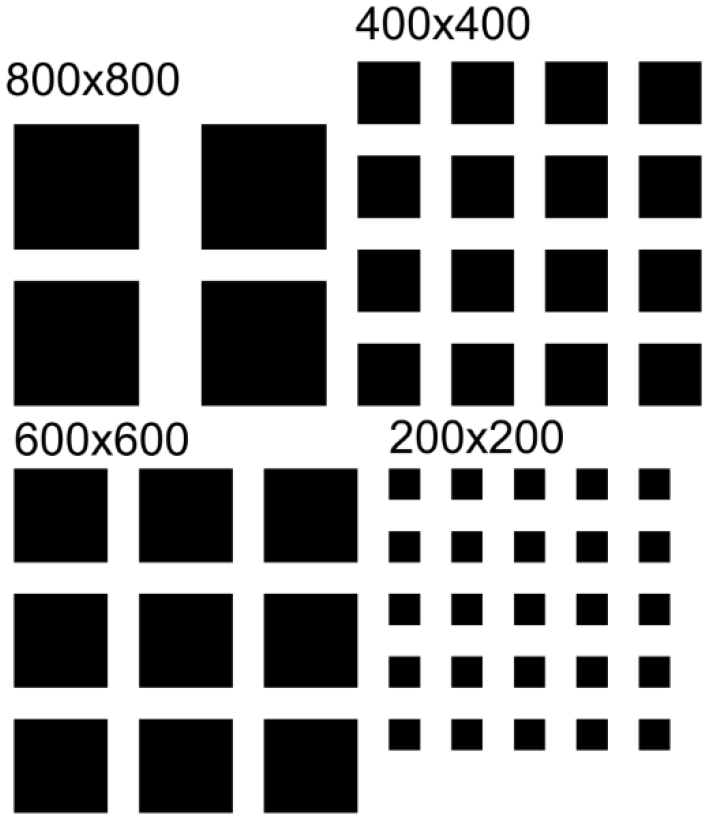
\includegraphics[width=0.4\textwidth]{Chapter3/Figs/3c.png}
\caption[Device Structure]{Device layout and dimensions of the top electrical contact.}
\label{fig:3c}
\end{figure}

\noindent To increase adhesion, a second titanium buffer layer is placed between the top metal contact and the oxide. This adhesive layer is less than ideal since it can cause additional imperfections to migrate within the oxide. Despite this worry, research using electron energy loss spectroscopy (EELS) and transmission electron microscopy (TEM) have shown no evidence of titanium interface migration in the devices \cite{mehonic2017intrinsic}. \\

\noindent It has been claimed that asymmetry in the device's construction, as well as an active and inert electrode, are necessary to identify stable switching. The molybdenum contact can be crucial as an oxygen reservoir, rapidly exchanging oxygen between the electrode and silicon oxide layer, which is similar to an active electrode, according to a recent experiment \cite{cox2021nanoscale}. The materials used for the top and bottom electrodes are different and weren't explicitly chosen for this project; rather, other group members had already picked them to create high-performance resistance switching memory. \\

\noindent The device layers remain mostly unchanged throughout the investigation. The top electrical contact is made of a different material in the experiment than the bottom electrical contact, which is made of a thin film of molybdenum. The oxide layer is made of an amorphous silicon oxide thin film. The selection of gold as the top electrical contact may cause gold atoms to diffuse through the film and migrate into the oxide. \\

\noindent Although gold has been seen to diffuse through silicon oxide layers at high temperatures, resistance switching memory frequently overlook this phenomenon or presume it does not happen. A profilometer is used to assess the thickness of the layers. To guarantee excellent conductivity throughout the device, the bottom electrode is 300 nm thick. The oxide slim film is 35nm in depth. The thickness of the top electrical contact varies depending on the substance; gold has a thickness of 110 nm, while ITO has a thickness of 50 nm.

RF sputtering, a physical vapour deposition process, was used to deposit all of the device layers. Deposition is carried out at low pressure in a typical inert gas environment by blasting the intended material with a plasma, which causes the expulsion of atoms from the target. Depending on the gas pressure inside the chamber, the expelled atoms either follow a direct ballistic path or take a random walk until they land on the sample. A greater gas pressure will result in more collisions and an increased random walk, whereas a lower gas pressure produces a more direct ballistic trajectory. \\

\noindent  The substance being deposited, known as the target material, is initially solid. By applying a strong electric field to the sputtering gas (argon), the plasma is created. Either a DC or an AC field is possible. However, an AC field that oscillates at an RF frequency of 13.56MHz is necessary for dielectric targets like SiO2. Sputtering often results in amorphous films with sub-stoichiometric oxides. The devices' SiOx oxide has a stoichiometry of 1.9, while the film's roughness appears to be determined by the RMS roughness of the underlying molybdenum layer, which ranges from 0.9 to 1.5 nm \cite{kenyon2019interplay}. \\

\noindent After being sputtered, film thickness is measured via a contact profilometer with a 0.5nm precision. During this procedure, a diamond tip is used to make contact with the sample and scan across the surface. Utilising a feedback loop, the tip's height is adjusted to maintain a consistent force against the sample's surface as it scans, giving the measurement of the sample height. The sample's surface height changes in direct proportion to the change in tip height. Layer thicknesses of a device stack are measured in relation to one another using a staircase-like pattern that is created during production.

\subsection[Electrical Characterisation]{Electrical Characterisation}

The amount of current passing through the device is a significant observable. This includes details on the oxide layer's bulk conductivity as well as the interface barrier heights. The difficulty, however, is in minimising any deviations or nonlinearities brought on by the measuring apparatus itself, with probe contact resistance serving as one such example. It is necessary to choose how to make contact with the device electrodes before conducting current measurements. There are essentially two methods: either the circuit is wire bonded inside a chip carrier, or the contacts are directly probed with tiny metallic probes using micromanipulators. \\

% \noindent In contrast to the probe method, which can be vulnerable to sample damage brought on by the experimentalist, the wire-bonded approach has the advantage which the position of the electrical connection does not change between experiments, thermal expansion while temperature measurements will not significantly affect the contact, and there is less risk of deteriorating the device throughout characterisation. However, there is a chance that the component will be broken during the bonding procedure with wires. An ultrasonic pulse is utilised to melt a gold or aluminium wire to the device contact while applying pressure to help fuse the two metals together. It has been regularly observed that this pressure can cause internal layers to compress, leading to electric shorts between the two metal contacts and ultimately damaging the device. \\ 

% \noindent The direct probing method utilising tungsten probes has been adopted instead due to the devices' design and susceptibility to break from the wire bonding procedure. The tip of the probe must be brought down carefully to prevent damage. When placing the probe into contact, a low voltage is often supplied as a test signal. To determine if the probe has made contact, the current is watched for a spike in the device current. Initially, because there is no measurable electrical current while the probe is not in touch with the device, the current oscillates around positive and negative currents at 0 amps. Once the probe makes contact with the device, the voltage that has been applied across it now causes a detectable current that matches the polarity of the applied voltage. \\

\noindent After deciding on a contact technique, the next choice is how currents will be monitored. Both a 2-wire measurement and a 4-wire measurement are frequently available as options. The sample's conductivity serves as the basis for the decision. The easiest way to measure electrical resistance is to apply a set voltage and track the total current passing through the object. Only two electrical connections are formed, thus the term "2-wire measurement" for this procedure. Ohm's Law is used to determine the device resistance by connecting a voltage source, an ammeter, and the device in series. \\

% \noindent Due to the assumption that the electrical resistance is only determined by the test device, which is not true in reality where there are several sources of electrical resistance connected in series with the device, this measurement is often not correct. These include the wires connecting the test object and the voltage source, the internal resistance of the voltage source or the ammeter, and, especially, the contact resistance that develops at the point where the electrical probes and the test object meet. \\

\noindent One of the most crucial parameters to take into account when describing thin films is contact resistance, which may be reduced by placing metal contacts on the sample during manufacturing. Fortunately, the device resistance usually outweighs the electrical resistance, making this method valid in the majority of instances. However, when resistance is small, the parasitic resistances of the measuring circuit become notable and must be eliminated by using a 4-wire resistance measurement. \\

% \noindent Ohm's law is still used in this configuration to calculate resistance. Instead of sourcing a voltage and monitoring a current, the device is subjected to a steady current that induces a voltage across it. Through two extra probes connected in parallel to the device, a voltmeter measures the potential decrease. It is crucial to recognise that the same contact resistance and wire resistances that plagued the 2-wire method continue to exist for all four connections. However, in this case, the high impedance of the voltmeter causes a substantially lesser current to pass through the measuring contacts. \\

% \noindent The voltage recorded by the voltmeter is thought to more precisely represent the voltage drop across the device since the voltage dip across the parasitic resistance is insignificant. This occurs because the voltage produced across the contact resistance is lowered as a result of the reduced current flowing through the probes, which detect the voltage across the device. By lowering these voltages, which are induced across each probe's contact resistances and contribute mistakes into the voltage measurements, it is possible to measure the voltage across the device with more accuracy.

\noindent Thus, the device resistance determines whether to use a 2-wire or 4-wire resistance measurement. The devices examined in this thesis have high resistance, ranging from kiloohms to megaohms. The parasitic resistances of the measuring circuit, like the contact resistances, are insignificant at this level. The issue of measuring device currents must now be solved once the device has been attached. Again, there are a variety of techniques that might be applied; the one selected will often depend on the size of the current being measured. \\

\noindent The average current range for the devices is 100nA to 1mA, therefore a picoammeter is required to detect considerably lower currents on the order of picoamps to nanoamps. Picoammeters minimise current readings by a number of methods that differ across manufacturers. The majority of them employ a transimpedance amplifier to magnify the signal while an op-amp converts the input current to a voltage. Once again, how this is implemented differs from manufacture to manufacture and is frequently protected intellectual property that is not revealed. The equipment used in this instance is the Keithley 6430 sourcemeter, which combines a picoammeter and a low noise voltage source into a single device. \\

\noindent In some cases, the device requires the application of voltage transients that are more complex than step potentials, such as pulses or custom spike trains. In these cases, the Keithley's sampling frequency is insufficient to generate such signals. An arbitrary signal generator is used in its place to create voltage transients, and a current preamplifier is connected in series with the device to amplify device currents. In particular, the oscilloscope (Rigol DS4024) and current preamplifier (SR570) are used.


\subsection[Device Stressing]{Device Stressing}

The method for reliably and repeatedly inducing the current transient phenomena is presented in this section. This not only enables the induction of current transients in a range of devices, but it also enables the progression of the transient from a barely detectable state to the dominant device activity. The approach described here has opened up the possibility of using the behaviour as a computational device while also enabling a more detailed characterisation of the behaviour. \\

\noindent Current transients were previously believed to be caused by oxide imperfections implying that if a device exhibits current transients, it only has to be designed as a faulty device. Fortunately, the fabrication and control of oxide defects is a current study area and is also known to as defect engineering. The act of applying sufficiently strong electric fields to a MIM device to cause a partial and reversible breakdown is known as electroforming. This is a common technique in memristor- and resistance-switching-memory (ReRAM)-based research, and it can also be simply seen in the silicon oxide devices utilised in this thesis.\\

\noindent Current transients were previously believed to be a result of oxide imperfections implying that if a device exhibits current transients, it essentially has to be designed as a faulty device. Fortunately, the fabrication and control of oxide defects is an ongoing research area and is also known to as defect engineering. The act of applying sufficiently powerful electric fields to a MIM device to cause a partial and reversible breakdown is known as electroforming. This is a common technique in memristor- and resistance-switching-memory (ReRAM)-based research, and it can also be simply seen in the silicon oxide devices utilised in this thesis.\\

% \noindent This makes electroforming a good place to begin when trying to introduce defects. But it's not flawless. Device conductance often experiences huge discrete jumps while electroforming. When devices go through this process, they display a switching behaviour across two states of resistance: one with high resistance and the other with low resistance. These discrete states are frequently highly stable. As a result, the qualities are significantly unlike from what we are familiar with about the transient, which is in contrast analogous and volatile. This begs the issue of how electroforming can be considered an effective approach to create transients when the final device behaviour is so different.\\

\noindent Observing that the conductance of a device showing transients is more comparable to the HRS of an electroformed device than to the LRS can provide insight into the link between electroforming and a current transient device. This led to the idea that, if a slightly more subtle electroforming technique were utilised, that is, before the major switching event, the current transient may be created. Because the electroforming process itself seems to be the outcome of a positive feedback mechanism, it is difficult to achieve a delicate electroformation \cite{kozicki2016electrochemical}.\\

\noindent When a voltage flows to the device, charge is injected into the oxide, creating defects such vacancies that increase the device conductance. This procedure has inherent instability. Higher current densities brought on by the increase in conductance speed up the creation of defects, which in turn causes current densities to keep rising until a catastrophic breakdown happens. When high constant voltages (13V to 15V) are supplied to the device, it is easiest to see this exponential rise in conductance. A regulated, gradual, and delicate modulation of device conductance is difficult to perform when this positive feedback effect dictates the change in conductance.\\

\noindent It is obvious that electroforming's fundamental positive feedback must be avoided. This is accomplished by abandoning voltage-based electroforming in favour of constant current electroforming, often known as "stressing the device" to distinguish it from the more widely used electroforming. A comparable voltage is provided at the peak of continuous current straining as is done during electroforming. The main distinction is that once the device begins breaking down, the voltage is reduced as a result of the current source's negative feedback. \\
% The time-dependent dielectric breakdown (TDDB) of oxides, which is caused by flaws in the insulator that increase conductance due to electron trapping, is frequently evaluated using the conventional approach of constant current stressing \cite{1487102}.

\noindent Instead of applying a set voltage, the device is provided with a constant current. This has the benefit of reducing the voltage across the device as it grows more conductive in order to maintain a constant current, which in turn delays the creation of oxide defects. This will go on once an equilibrium is established when the applied voltage is decreased to a level where formation no longer takes place, but is still great enough to keep the continuous current flowing. Now that the process presents negative feedback, it is considerably more conducive to causing subtle alterations in device conductance. \\

\begin{figure}[htbp!] 
\centering    
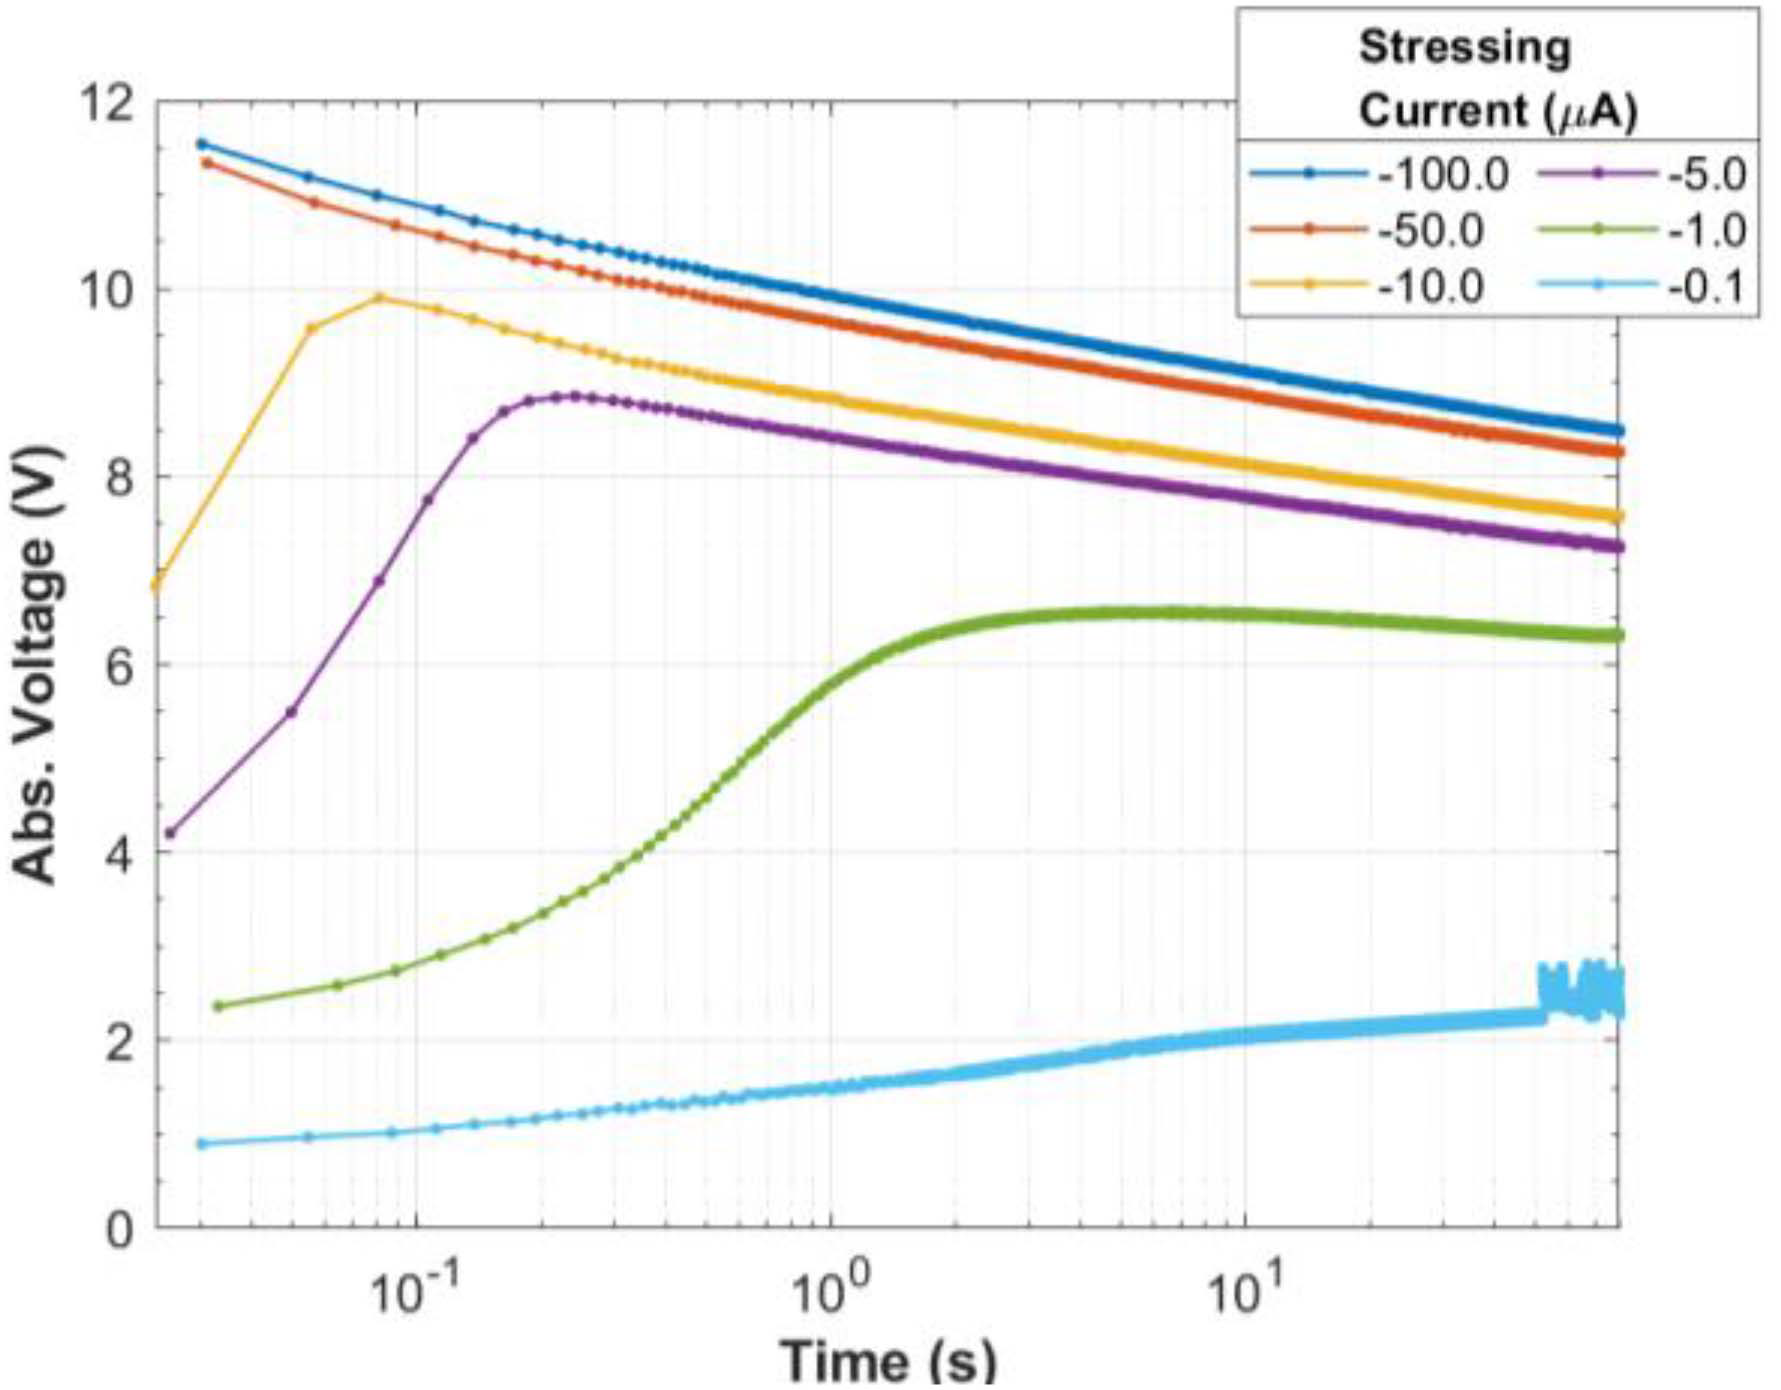
\includegraphics[width=0.6\textwidth]{Chapter3/Figs/3d.png}
\caption[Response of devices to different magnitudes of stressing currents.]{The device's voltage is recorded while subject to constant current stress, with six devices tested at various current levels. The voltage across each device is plotted during the initial constant current stress for six devices, each with a different current magnitude.}
\label{fig:3d}
\end{figure}

\noindent Essentially, the devices are subjected to stress by grounding the molybdenum contact and applying negative currents to the gold contact, resulting in electron injection at the gold contact and hole injection at the molybdenum contact. The magnitude of the constant current is adjusted based on the desired behaviour, with values ranging from $-0.1\mu A$ to $-100\mu A$ for a duration of 100 seconds. During stressing, the voltage induced across the device gradually decreases, eventually reaching a steady state value as shown in Figure \ref{fig:3d}.\\

\noindent It's important to take into account that after being stressed, the device doesn't immediately display the current transient. The relaxation process can be accelerated by providing a positive potential to the above gold-titanium contact, but it must still be allowed to rest for 24 hours. When allowed to rest, the device will eventually show current transients. This delayed response is not unexpected as a result of a drifting defect with restricted mobility. While the generated defects are still present, the relaxation time allows this to return to its resting distribution at thermal equilibrium. It is expected that the stressing results in significant drifting and defect generation.

\subsection[Induced Transient]{Induced Transient}

The established method enables the induction of current transients in devices, and it may be done so gradually. The prominence of the current transient can be altered when the devices are subjected to varying levels of stress by varying the current's magnitude. To be more precise, a device's current peak becomes more evident the more stressed it is. It was previously claimed that this was caused by the thinner devices' higher current densities masking the current transient \cite{el2007ionic}. \\

\noindent Instead of looking at current densities, a possible reason of the prominence of current transients may be based on the total number of defects present in the oxide. It follows that thicker devices will have more defects overall if it is assumed that the concentration of defects in the oxide layer remains relatively constant throughout growth. In this instance, it is also assumed that more oxide defects will be produced the more aggressively the device is stressed. Therefore, it is possible that the total number of defects present in the oxide, rather than the conductance of the device, can be used to predict the transient's amplitude. \\

\noindent A device being stressed does not ensure that there will be current transients. As soon as electrons are introduced at the top gold-titanium contact, the device only displays current transients when it is stressed with negative currents. The response is different when electrons are injected at the molybdenum contact. The structural alterations that stressing causes in the device can be used as evidence for the reason only negative currents can cause current transients. As anticipated, the stressing process results in structural flaws at the electrical contact, as has been seen in the past when comparable devices were electroformed and switched repeatedly \cite{waser1990dcI,waser1990dcII}. \\

\noindent Negative currents are used to stress devices, which involves grounding the molybdenum contact while applying negative voltages to the gold contact to inject electrons into the oxide. This causes a high number of tiny holes to form in the contact, which are often clustered together in one area. It is unclear where these traits came from. Since the specific area where the faults are present does not match the location of the probe on the object being examined, a mechanical explanation is ruled out. \\

\noindent When the device is strained with positive currents, or electrons are introduced into the molybdenum contact, noticeably distinct faults are generated. The overall contact looks to get rougher, not just the individual holes. The flaws in this instance are repeatable across devices and cover practically the whole contact. It should be emphasised, nevertheless, that these flaws are not necessary for observing current transients, and they were avoided in the devices examined here.

\section[Results]{Results}

Current transients are difficult to define because they are elusive, sometimes mistaken for faults, and only seen in a small number of the devices in a batch. This is due in part to the difficulty of developing devices that reliably produce transients. It is ideal to be able to gradually create an effect and link its presence to any changes in device attributes in order to define a behaviour in detail. It is understandable that the analysis that could be done was restricted since published research on current transients relies on the irregular appearance of current transients. Therefore, it is obvious that the lack of a method to create transients is a crucial tool if we are to fully comprehend this phenomena.

\subsection[Neuromorphic Behaviours]{Neuromorphic Behaviours}

In essence, the behaviour of the current transient phenomenon can represent the ability to exhibit both analogue potentiation and depression under the same voltage polarity and amplitude. Potentiation and depression are two fundamental processes that occur within synapses and are the foundations of more complex learning rules. During potentiation, a synapse's conductivity increases, whilst during depression, it decreases. \\

\noindent Changes caused during potentiation or depression can also vary in volatility: they may persist and be long-term (Long-Term Potentiation (LTP) and Long-Term Depression (LTD)) or their effects can reverse over time and be considered short-term (Short-Term Potentiation). be regarded as short-term (Short Term Potentiation (STP) and Short Term Depression (STD)).\\

% \noindent These fundamental synaptic behaviours have been replicated in a wide variety of electronic devices, predominantly memristors or ReRAM devices, which have been shown to exhibit both potentiation and depression over both long and short timescales \cite{jo2010nanoscale}. However, in these examples, potentiation and depression often occur in opposite polarities. This necessitates that enhancing and reducing inputs should be capable of producing spikes of varying polarities, which could result in a rise in intricacy of the neuron circuits that govern the synapses.\\

% \noindent It would be advantageous to construct networks that can operate on a single rail power supply similar to the majority of modern digital electronics. Achieving this would necessitate the use of devices in which potentiation and depression can occur solely as a result of a single polarity of voltage pulse. There are instances of devices displaying potentiation and depression within the same voltage polarity, including complementary ReRAM \cite{khan2020comparison} or unipolar ReRAM devices \cite{mehonic2012electrically}. Nevertheless, these devices demonstrate discrete binary switching behaviours, rather than the more biologically analogous analogue changes in resistance.\\

\begin{figure}[htbp!] 
\centering    
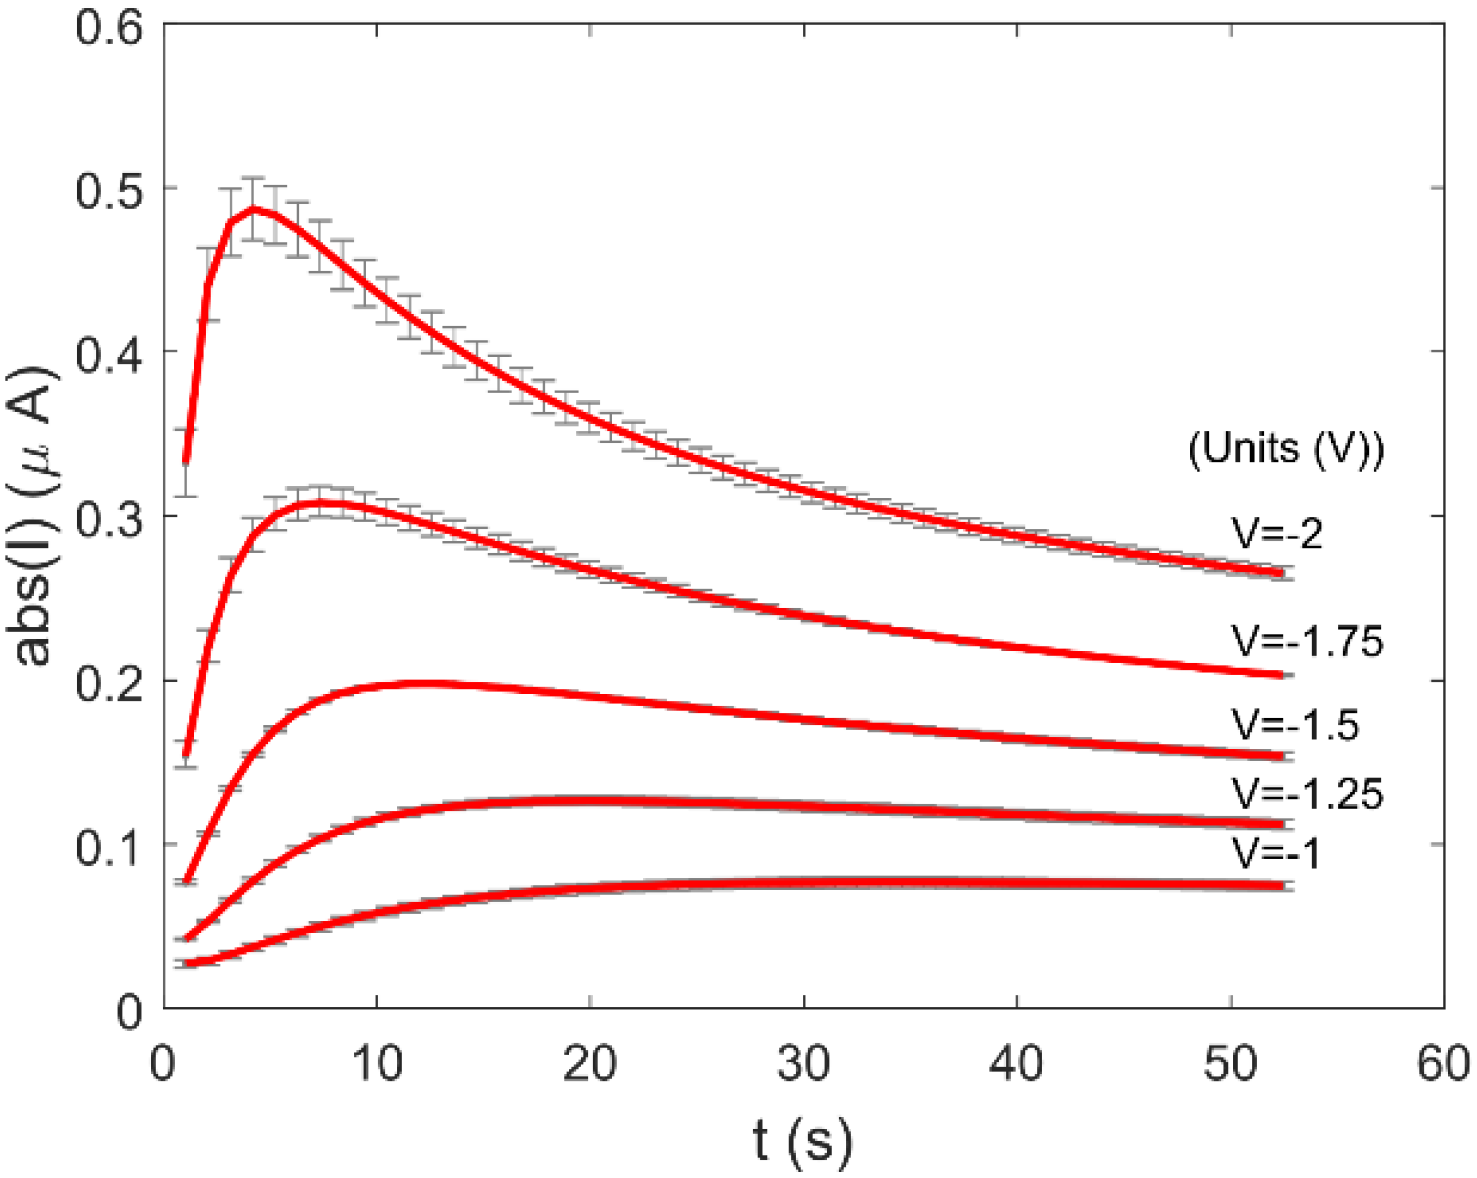
\includegraphics[width=0.5\textwidth]{Chapter3/Figs/3e.png}
\caption[The voltage dependence of the current transient in the subthreshold regime.]{The transient currents of amorphous silicon dioxide thin films were analysed for various voltages. The voltage is applied to the gold electrical contact while the molybdenum contact is grounded. For each voltage, the average of three trials is recorded and presented graphically, with error bars indicating the range of the three trials.}
\label{fig:3e}
\end{figure}

\noindent The device's potentiation and depression can be best demonstrated by applying a step potential. When a negative step potential is applied to the top gold electrode of the device, transient current is observed, as shown in Figure \ref{fig:3e}. Initially, a rapid potentiation occurs, taking just a few seconds, but it quickly reaches a peak beyond which the depression phase begins. The device conductance is gradually dominated by competition with depression, ultimately causing the conductance to fall below its original level.  This occurs over a longer period of time, lasting tens of seconds and continuing for tens of minutes.\\

\noindent The transient current response of the device to a range of DC voltages is plotted in Figure \ref{fig:3e}. For each voltage the mean of 3 trials is plotted, with error bars indicating the maximum and minimum of all trials. At lower voltages, i.e. -1 V, negligible depression is observed, but it becomes progressively more prominent at larger voltages. Potentiation is observed for all voltages, including -1V, and appears to accelerate with increasing voltage.\\

\begin{figure}[htbp!] 
\centering    
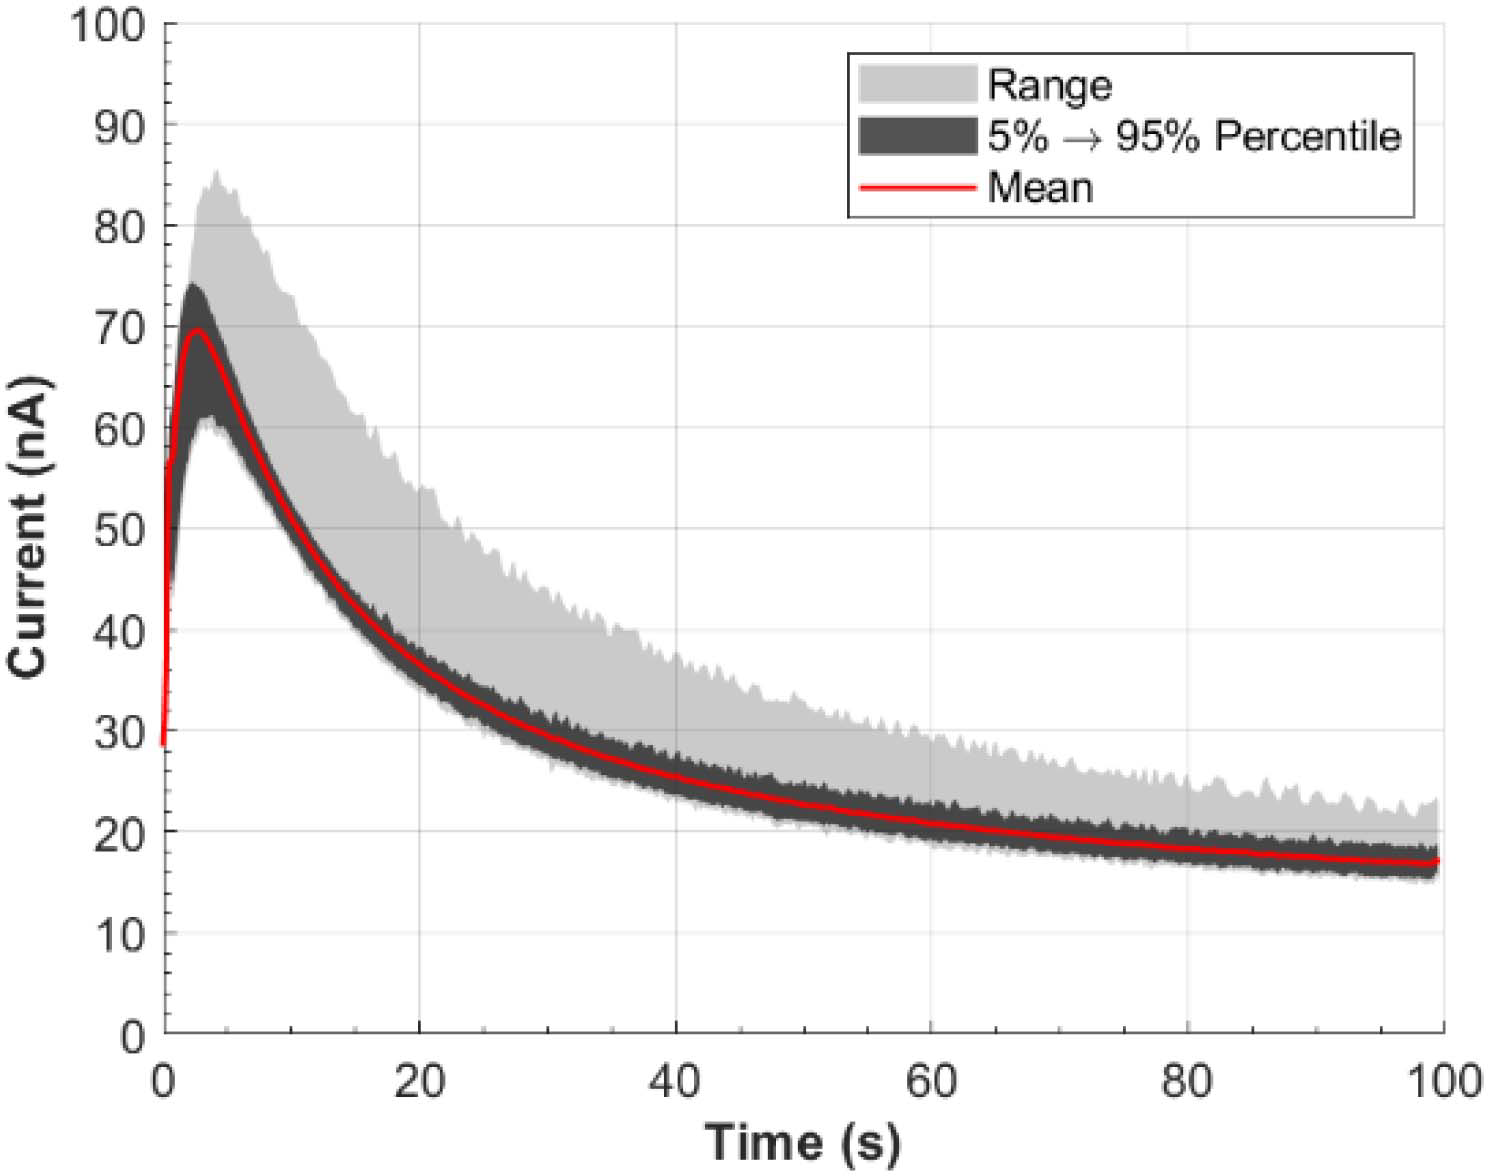
\includegraphics[width=0.5\textwidth]{Chapter3/Figs/3f.png}
\caption[Repeatability of current transients in the sub-threshold range.]{The mean, range and 5th - 95th percentiles are presented graphically for 132 current transients that were induced by applying a -0.8 V step potential to the gold electrical contact while the molybdenum was electrically grounded. A single-order low pass filter with a cutoff frequency of 10 kHz was applied to the data to eliminate noise that may mask the variation between trials.}
\label{fig:3f}
\end{figure}

\noindent It is worth highlighting the repeatability of the device's response as presented in Figure \ref{fig:3f}, where a collection of 132 current transients induced by a step potential of -0.8 V applied to the gold electrical contact is displayed. Although resistance switching devices frequently display variable and stochastic responses, it is apparent that the device's performance is consistent and foreseeable, as demonstrated by the range (light grey) and the 5th and 95th percentiles (dark grey). The range has a wider spread than the 5th and 95th percentiles, attributed to bigger currents observed in the first three trials, resulting from a settling process across numerous trials.\\

\noindent This statement only holds true if the device is allowed to fully relax between trials. To achieve relaxation, both electrical contacts should be grounded and the device left to rest. The reset process is gradual, necessitating a resting period of one hour to guarantee complete relaxation. Accelerated relaxation can be attained by applying a positive potential to the gold contact, as opposed to grounding it.\\

\noindent While this behaviour is noticeable during step potentials, it is crucial to examine whether the same behaviour can be reproduced when operating neuromorphic synapses using pulse trains. We demonstrate that this is achievable by administering a sequence of Gaussian pulses to the appliance. The pulses have a full width half maximum (FWHM) of 20 ms, an amplitude of -3 V, a period of 300 ms, and are once more implemented on the gold contact. Note, while the pulses have a negative amplitude, the device current has been inverted in the following figures to enhance clarity.\\

\begin{figure}[htbp!] 
\centering    
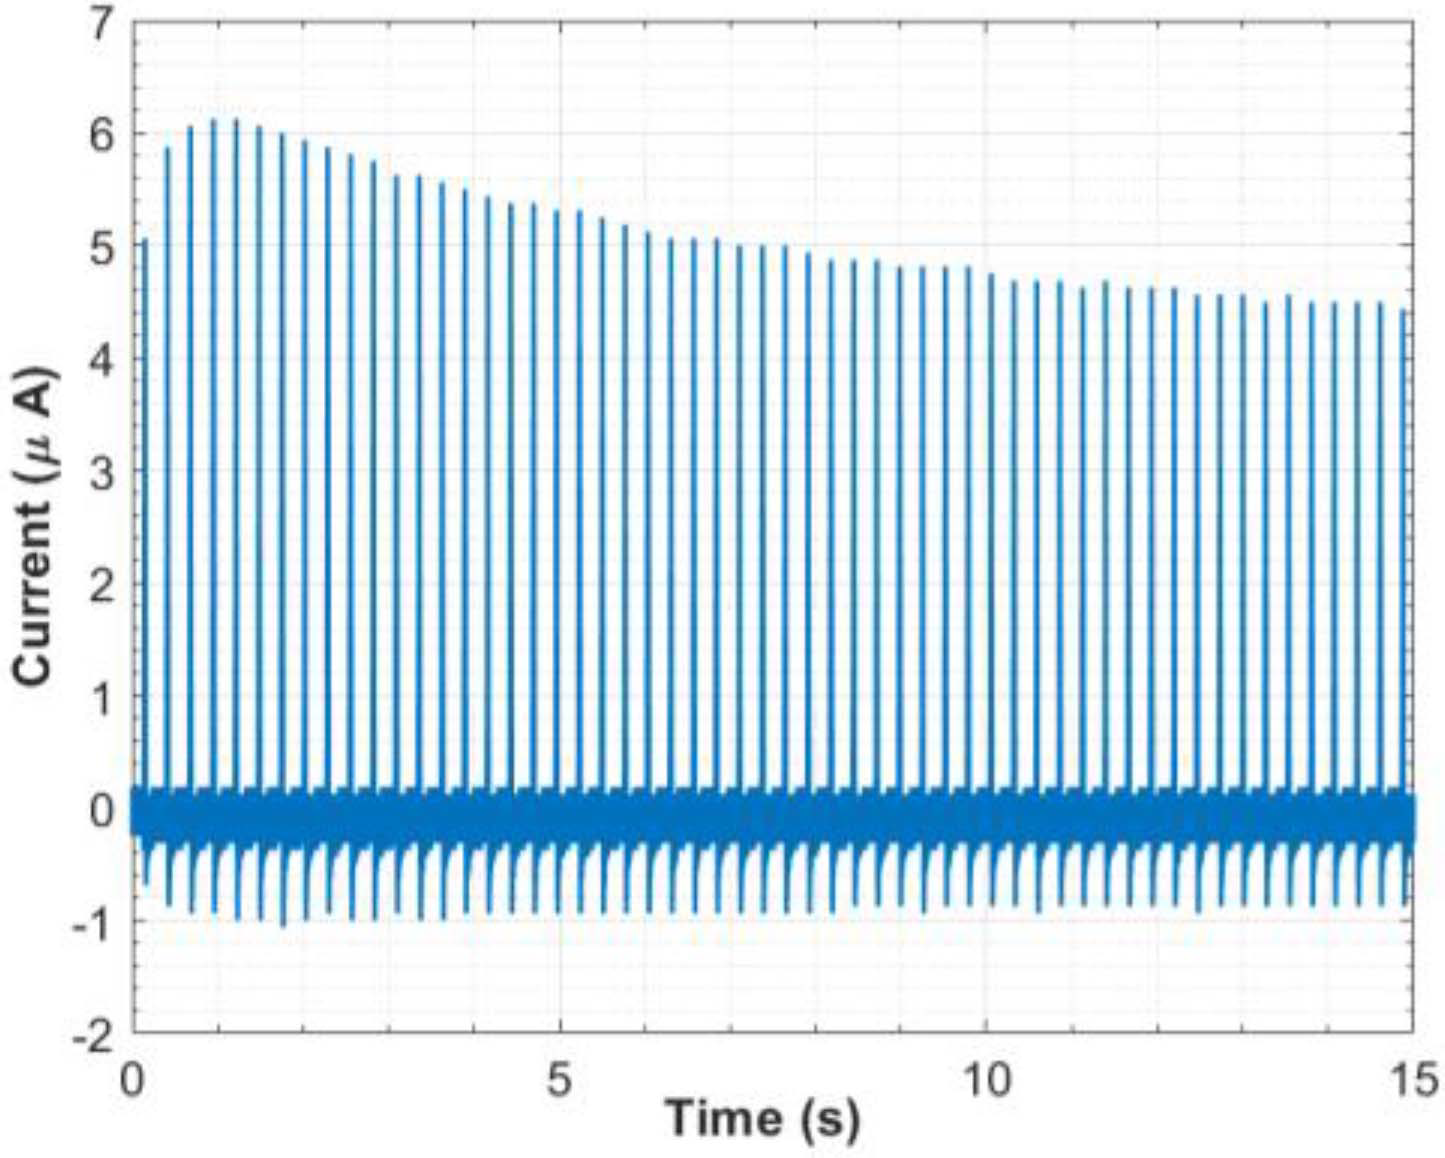
\includegraphics[width=0.5\textwidth]{Chapter3/Figs/3g.png}
\caption[Device response to a spike train.]{The current that passes through the device while a spike train is applied is measured. The pulses are applied to the gold electrical contact while the molybdenum contact is grounded. Each pulse has a Gaussian form with a Full Width at Half Maximum (FWHM) of 20 ms, an amplitude of -3V, and a period of 300 ms. The magnitude of the current has been inverted for clarity. The device was electrically stressed with a constant current of $-100\mu A$ for 100 seconds.}
\label{fig:3g}
\end{figure}

\noindent The response to the series of Gaussian pulses is shown in Figure \ref{fig:3g}, indicating a behaviour similar to that in the DC measurements. An initial potentiation lasting about four pulses is followed by a longer depression period. This indicates that a combination of potentiation and depression can be achieved in both DC and spike train operation, promising the suitability of the device for use in spiking neural networks.\\

\noindent One possible advantage of the subthreshold regime lies in its substantial resistance value (approximately 10 M$\Omega$). Typically, resistance switching devices applied for neuromorphic computing alternate between high resistance states (about 100k$\Omega$) and low resistance states (about 1k$\Omega$). \\

\noindent Nevertheless, in the subthreshold regime, our device remains within a range of resistances comparable to or even higher than the high resistance state of binary resistance switching devices. This indicates that the device may function with lower current consumption than a typical resistance switching device.\\

\noindent However, it must be acknowledged that inherent limitations exist. The broad range of resistance in switching devices reduces their sensitivity to noise or voltage fluctuations, while also enabling a wider range for programming. Thus, there exists a trade-off between current draw and resistance to noise. Additionally, the subthreshold regime poses the challenge of voltage dependency in depression mechanisms. As depicted in Figure \ref{fig:3e}, depression is seldom observed below -1V. This, in turn, constraints the operating voltage of subthreshold circuitry wishing to utilize depression dynamics.\\


\subsection[Transient Tunability]{Transient Tunability}

The capability to choose between potentiation and depression is crucial for circuit designers who intend to exploit the device in neuromorphic circuits. The more adaptable approach is to regulate the magnitude of the applied pulses. Figure \ref{fig:3e} demonstrates that lower voltages, such as -1V, display a certain level of potentiation but not depression. This is also true for low-voltage spike trains.\\

\begin{figure}[htbp!] 
\centering    
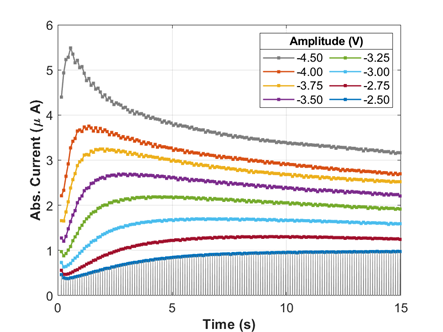
\includegraphics[width=0.5\textwidth]{Chapter3/Figs/3h.png}
\caption[Dependence of potentiation and depression on the amplitude of applied voltage pulses.]{The plot illustrates the device current for Gaussian spike trains with increasing amplitude. Grey-coloured Gaussian current pulses represent the smallest amplitude (-2.5 V). To improve clarity, only the peaks of each pulse are plotted for higher amplitudes. The pulses have a Full-Width at Half-Maximum (FWHM) of 20 ms and a period of 100 ms. Priorly, the device underwent electrical stress when exposed to a constant current of -50$\mu$A for 100 seconds.}
\label{fig:3h}
\end{figure}

\noindent Figure \ref{fig:3h} depicts the current response to spike trains of varying pulse amplitudes. Depression is not observed with lower voltages. It is possible that the absence of depression at lower voltages indicates a threshold electric field required to induce the change from potentiation. This implies overcoming an activation barrier to initiate defect drift.\\

\noindent On the contrary, depression may be the intended response. In this instance, the amplitude of impulses may be raised to the point where the initial potentiation is overcome. Figure \ref{fig:3i} depicts the percentage upsurge in device conductance from its initial value. The experiment is replicated for spike trains of differing amplitudes. It can be seen that spike trains with an amplitude < -3.75V are largely potentiating, with the change in conductance remaining positive. However, when the amplitude is increased to -4.5 V, the spike train leads to negative changes in conductance, resulting in depression.\\

\begin{figure}[htbp!] 
\centering    
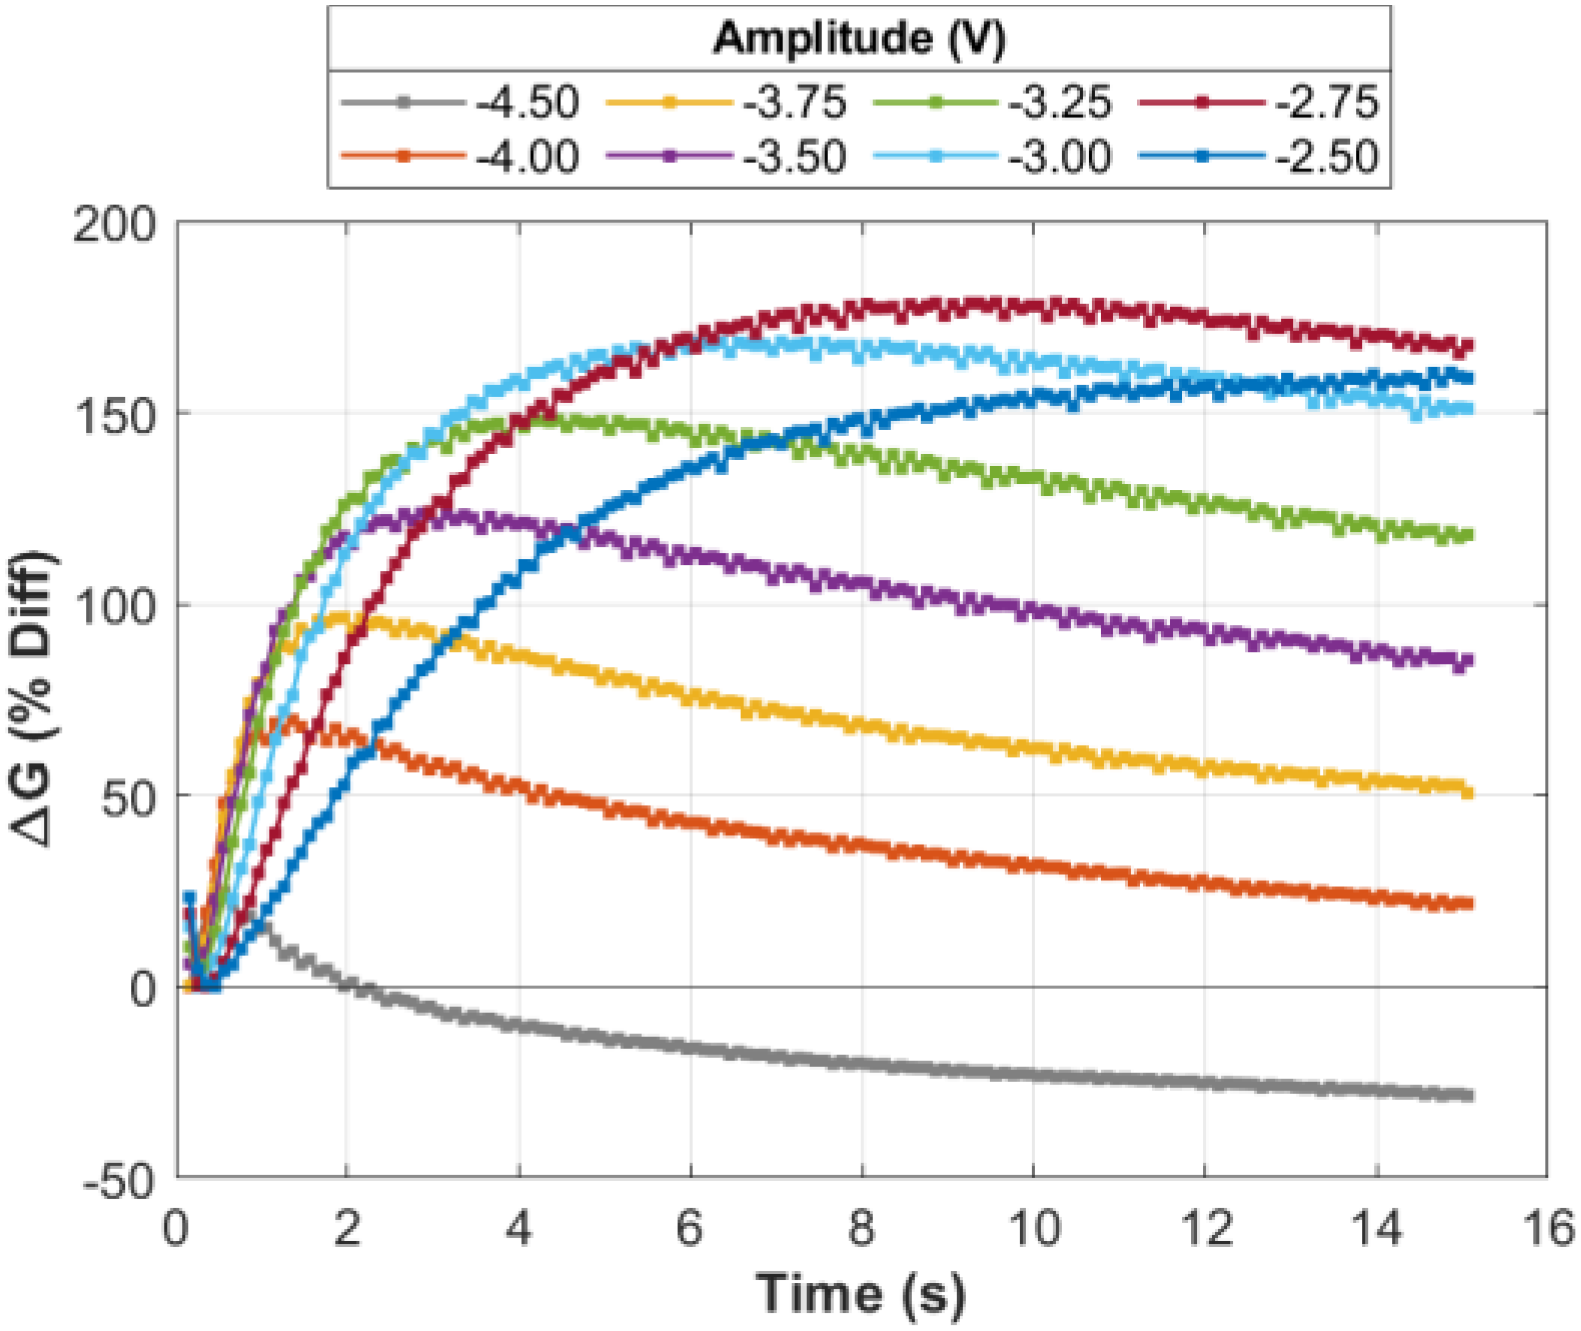
\includegraphics[width=0.5\textwidth]{Chapter3/Figs/3i.png}
\caption[Depression selection using spike trains of greater amplitudes.]{The percentage difference in conductance caused by each spike train pulse is represented on a graph. Larger amplitudes mainly cause depression, whereas smaller amplitudes lead to potentiation. Before testing, the device underwent electrical stress through a constant current of -50$\mu$A for 100 seconds.}
\label{fig:3i}
\end{figure}

\noindent An alternative and enduring method to select a particular behaviour is to modify the electrical stress that the device experiences after production. As outlined earlier, the devices undergo initial stress through the application of a constant current to the device. The current magnitude is modifiable, which, in turn, alters the degree of stress imposed on the device, thereby allowing adjustment of the device's current transient response. In figure \ref{fig:3d}, the response to stress is then plotted for six different devices, with each being subjected to varying currents ranging from -0.1 $\mu$A to -100 $\mu$A. Each device is subjected to the current for 100 seconds.\\

\begin{figure}[htbp!] 
\centering    
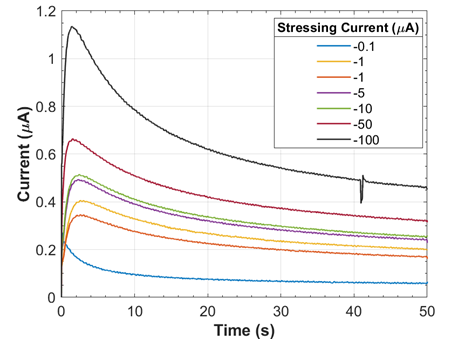
\includegraphics[width=0.5\textwidth]{Chapter3/Figs/3j.png}
\caption[Device current dependence on stressing magnitudes.]{The device current is plotted in response to a step potential of -1.25V for devices initially stressed to varying degrees. There is no potentiation in devices stressed to a lesser extent, while heavily stressed devices exhibit greater potentiation and depression. For clarity, the absolute value of the device current has been plotted.}
\label{fig:3j}
\end{figure}

\noindent The resulting current transients display a noticeable potentiation for higher stressing currents, accompanied by an increasing conductance. However, the device stressed with the smallest current, -0.1$\mu$A, shows no potentiation, only depression. Conversely, the device exposed to the maximum current, -100$\mu$A, potentiates up to almost 10 times its initial conductance.\\

\noindent These methods offer the chance to modify the level of potentiation taking place in the device, ranging from minimal to noticeable. It is crucial to observe that this adjustment is irreversible and would typically be determined during circuit manufacture. In contrast, the method of altering spike amplitude is adaptable and can be modified while in use.\\

\noindent Given the device's ability to display both an increase and decrease in conductance, each occurring at varying rates and with different relaxation rates, it is unavoidable that the steady state conductance will differ across various spike train periods. Before investigating the computational potential of this behaviour, it must first be confirmed.\\

\begin{figure}[htbp!] 
\centering    
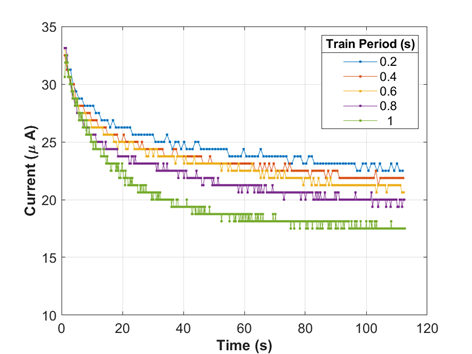
\includegraphics[width=0.5\textwidth]{Chapter3/Figs/3k.png}
\caption[Device suitable for trains of voltage spikes with varying inter-spike time periods.]{The device's maximum current is graphed for each pulse applied to a 400 by 400 $\mu$m device. The pulses take the shape of a Gaussian curve with a FWHM of 50 ms and an amplitude of -2.25 V. For clarity, the absolute value of the device's current has been shown.}
\label{fig:3k}
\end{figure}


\noindent In Figure \ref{fig:3k}, a graph plots the device current produced by spike trains with varying inter-spike time periods. The device ultimately settles into a steady state conductance in response to each spike train, where conductance changes induced by the applied spikes are counterbalanced by the device's relaxation dynamics. As anticipated, the steady state conductance is found to be dependent on the frequency of the pulses applied to the device - higher frequency pulses lead to decreased conductivity. These findings imply that this conduct could potentially be utilised to adjust the device resistance in response to spike trains of different frequencies. 

\subsection[Homeostasis Applications]{Homeostasis Applications}

\noindent The original aim of this study was to illustrate the potential application of distinctive memristive device behaviour for innovative computing architectures. One noteworthy application to emphasise is the neuron's capacity to adjust based on a firing frequency analogous to homeostasis in biology \cite{tien2018homeostatic}. \\

\noindent In biological systems, homeostasis refers to the maintenance of preferred operating conditions or particular states \cite{turrigiano1999homeostatic}. An example of this is the regulation of body temperature. When applied to spiking neural networks, homeostasis plays a role in maintaining spiking activity to avoid excessive power consumption through unnecessary spike events. It can also protect against faulty neurons entering a chaotic, high-activity state. Without homeostasis, such events could cause the entire network to enter a chaotic state \cite{marder2006variability}. \\

\noindent This process is also known as habituation, a type of homeostasis in which a change in input results in a temporary change in output that eventually diminishes to a steady-state value. There are already a few practical examples of this in recurrent neural networks, one of which resulted in a 20\% improvement in classification accuracy on the MNIST dataset when compared to a neural network without homeostasis.\\

\begin{figure}[htbp!] 
\centering    
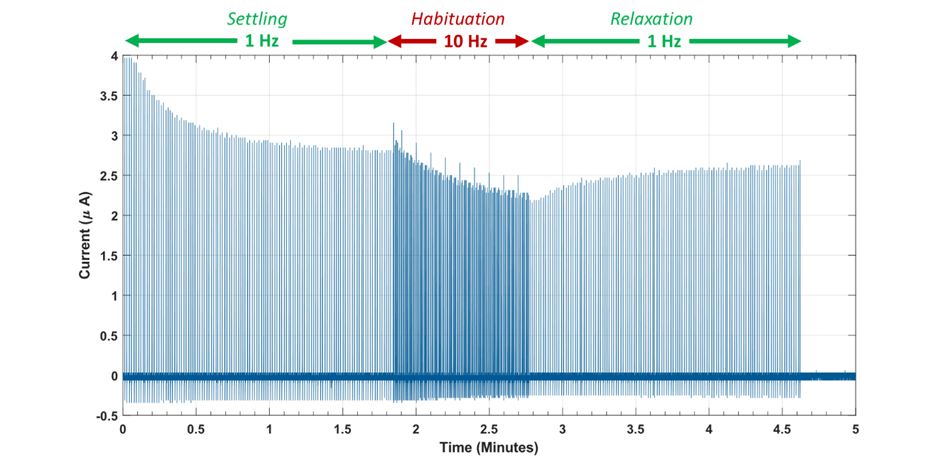
\includegraphics[width=1\textwidth]{Chapter3/Figs/3l.png}
\caption[Response of the device to different frequency of spike pulses]{Response of the device to varying frequencies of spike pulses. The device was initially operated with a sequence of 1Hz spike pulses, followed by a period of 10Hz spike pulses, before finally returning to 1Hz spike pulses.}
\label{fig:3l}
\end{figure}

\noindent The previous section showed that the steady state conductance of the device is reliant on the firing rate of the related neuron. The device conductance decreases at higher spiking frequencies, but has a greater steady state at lower frequencies. This behaviour is suitable for inhibiting the impact of suboptimal input neurons that have entered into a chaotic state of high frequency.\\

\noindent Figure \ref{fig:3l} demonstrates this concept in practice. The unit is connected to a signal generator that produces Gaussian pulses with a low frequency of 1Hz, which is the neuron's typical background activity. In these conditions, the device attains a steady-state conductivity. An input neuron is simulated as transitioning to a dysfunctional state of higher activity at t = 1.8 minutes, potentially caused by circuit damage. The frequency of the spike train is increased to 10Hz. \\

\noindent Without homeostasis, this mistaken input could cause the linked output neuron to reach a comparable state, which could then transmit through subsequent layers of the neural network. Luckily, when subjected to the high-frequency spike train, the conductivity of the device reduces due to the enduring behaviour of the current transient device. This decreases the overall current supplied to the linked output neuron, decreasing the chance of this high-frequency input triggering equivalent actions in the following neurons.\\

\noindent  While the temporary suppression is advantageous for safeguarding the network against excessive firing, it should not be a permanent solution. If the input neuron recovers to normal functional conditions, the inhibition should be lifted, and the neuron should be allowed to resume its place in the network. At t = 2.8 minutes, evidence was presented to support this idea. With a 1Hz spike train, the sample recovers to the background level of activity. The device conductance responds to the fluctuation of current transient conductance changes by returning to its former steady state value prior to the neuron's faulty phase. \\

\noindent The ability of protective systems to return to their original state when normal operating conditions are restored is a fundamental characteristic of homeostatic processes. Although the concept of homeostatic habituation has been demonstrated with the current temporary device, there are still limitations. For instance, it is impossible to determine a specific and constant conductance value while the device is operating in its present transient state. If the device is electroformed similar to a regular memristor, it allows for the weight to be adjusted to a variety of analogue values.\\

\noindent To achieve homeostatic behaviour in a physical system, it may be necessary to connect the device in series with another device that is programmable. The good news is that the programmable device and the current transient device are architecturally identical and manufactured using the same method. The devices can be combined on a single wafer since the only difference between them is the method in which they are electrically stressed.

\subsection[Physical Implications]{Physical Implications}

Initially it was thought that the transient was the consequence of an ionic current superimposed on an electronic current \cite{many1962theory, lampert1970current}. The ionic current is the outcome of a field-driven drift of some space charge, which is often assumed to be charged oxygen vacancies in more recent research \cite{saha2001transient}. The variations in conductance seem to stem from two distinct modifications happening simultaneously in the sample. An ionic current could only account for this observation if the drifting space charge were capable of drifting at a constant velocity permanently. \\

\noindent A more appropriate explanation is that the transient is an electronic current that is altered by changes in the device's conductance, with two simultaneous changes causing the transient \cite{meyer2005oxygen}. This is because the electronic conductance of an MIM device can be modified in several ways, some of which may occur simultaneously. The literature review identifies a general trend favouring an electronic explanation over an ionic explanation. \\

\noindent There are, however, numerous mechanisms through which the electrical conduction of an MIM device can be adjusted. An MIM device can be abstracted as a series combination of three distinct components: a metal-insulator interface, a bulk insulator, and a second metal-insulator interface. These components determine the device's conductance; however, in specific cases, one of these three components may be significantly more resistive than the others. In such circumstances, that particular component alone may provide a good estimate of the device's conductance. \\

\noindent So far, there has been no research to determine which layer, if any, dominates the conductance of a device that shows current transients. Most devices described in literature display rectifying behaviour, implying an interface-defined conductance. However, it is important to note that even if a device is rectifying, this does not necessarily indicate that the dynamics are always accurately described by an interface model. \\

\noindent In the reverse polarity, when the interface exhibits the least conductivity, the conductance of the device can be accurately captured by the interface model, since it is expected to have high resistivity. However, in the forward polarity, when the interface is most conductive, the bulk oxide may have a greater impact on describing the device conductance, necessitating a bulk-based model. Without knowledge of which layers define the device conductance, it is necessary to investigate every layer within the device to determine the physical changes that could be causing the current transients. \\

\noindent The bulk oxide, where the crystalline oxide is highly insulating as a result of the oxide's large bandgap. At high voltage and low temperature, current through the oxide occurs predominately via tunnelling- either directly or via the Fowler-Nordheim mechanism from Table \ref{table:1a}. However, the presence of electron trap states within the oxide results in the possibility for higher current densities through the use of these traps as alternative conduction pathways. \\

\noindent This thesis examines a sample of amorphous silicon oxide. Such oxides contain a higher concentration of oxygen vacancies, which affect electronic conduction by acting as electron/hole traps. Additionally, these oxides have an efficient pathway to creating oxygen vacancies. In the amorphous phase, the silicon dioxide has wide $O-Si-O$ bond angles \cite{el2013identification}.\\

\noindent The sites can trap a maximum of two electrons in this broad bond, which decreases the energy barrier required to generate the vacancy \cite{gao2016mechanism}. The existence of oxygen vacancies and an efficient route to their generation results in the degradation of the oxide. Conduction takes place via vacancy trap sites despite the wide bandgap. \\

\noindent There is evidence of the formation of conductive bridges through the oxide via trap states according to TEM \cite{munde2017intrinsic, wu2015evolution} and CAFM \cite{buckwell2015conductance} etching techniques. At higher temperatures, trapped electrons can be excited from one trap state within the bandgap to its neighbour, or across the oxide through the conduction band, via Poole-Frenkel conduction due to thermionic emission within these states \cite{frenkel1938pre}.

\begin{align}
    \sigma_{PF} &= q \mu_n n_{PF} = q \mu_n n_0 \left( \frac{-q (\Phi_B - \Delta\Phi_{PF}) }{k_B T} \right) \label{eq:3.14} \\
    j_{PF} &= E \sigma_{PF} = E q \mu_n n_0 \left( \frac{-q (\Phi_B - \Delta\Phi_{PF}) }{k_B T} \right) \label{eq:3.15}
\end{align}

\noindent The Poole-Frenkel effect raises the conductance of an oxide, $\sigma_{PF}$, by increasing the amount of free electrons in the conduction band relative to its thermal equilibrium concentration, $n_0$ to $n_{PF}$. The applied field reduces the barrier height, $\Phi_B$, necessary for an electron to be thermally excited from its trap state into the conduction band, causing this rise. For an applied field, $E$ and equation (\ref{eq:3.15}) where $\Delta \Phi_{PF} = \sqrt{\frac{q^3 E}{\pi \epsilon}}$, the drop in barrier height represents the increase in conductance produced by the reduction in barrier height \cite{sze2021physics}. Because this impact is reliant on the thermal energy of the electron, the number of extra electrons is based on a Boltzmann distribution and is determined by the thermal energy, $k_B T$, of the electron. \\

\noindent It is evident that the conductance of a device, regulated by the Poole-Frenkel effect, may be influenced by a change in the carrier concentration of the trap sites, $n_0$, and a reduction in barrier height, which varies with the local electric field, $E$. Both of these factors will be considered when examining the model as a potential explanation for current transients.\\

\noindent Poole-Frenkel, however, is not the sole cause of conductivity through trap sites \cite{dimaria1995mechanism}. The transfer between proximate traps can occur via tunneling, termed trap-assisted tunnelling (TAT) \cite{jimenez2001physical}. This method has already been proven to sufficiently account for conduction in amorphous silicon dioxide sheets showing resistance switching behaviour \cite{mehonic2012resistive}. One potential TAT model is founded on an inelastic tunneling process, ITAT \cite{ielmini2000modelingII}.\\

\noindent Both the Poole-Frenkel and ITAT models are capable of explaining the alterations in conductance witnessed during the current transient. The rise in conductivity, which is probably due to charge trapping, can be effectively accounted for by these models. Take, for instance, the Poole-Frenkel model (\ref{eq:3.15}), in which the current of the device results from the trap population, $n_0$, and the likelihood of an electron making a thermal leap from the trap to the conduction band. The model details steady-state conditions, where the trap populations remain constant.

\begin{align}
    E(x) &= \frac{V}{d} \label{eq:3.16} \\
    E(x) &= \frac{V}{d} - \frac{Qx}{\epsilon d} \label{eq:3.17}\\
    E(x) &= \begin{cases}
\frac{V}{d} - \frac{Qx}{\epsilon \delta} & \text{ if } x< \delta \\ 
\frac{V}{d} - \frac{Q}{\epsilon} & \text{ if } x\geq \delta 
\end{cases} \label{eq:3.18}
\end{align}

\noindent It is conceivable, though, that this term could be treated as time-dependent. At first, with the device grounded and at room temperature, the traps may be largely depleted, corresponding to the low conductance observed when the step voltage was first applied to the device. With the voltage now applied, however, traps that were previously depleted or had a low probability of being filled when grounded may now have a higher probability of being filled, corresponding to an increase in the probability of a trap being filled, $n_0$.\\

\noindent As the device becomes more conductive and higher current densities flow through it, the number of electrons trapped within the oxide increases. This eventually leads to a higher equilibrium or steady state value of $n$. A similar argument can be made for the ITAT model, which acknowledges that the probability of traps being populated varies with time and already accommodates transient effects. In order to observe an increase in conductance, the current flowing into the traps must exceed the current flowing out of the traps.\\

\noindent The decline in conductance may also be accounted for by positing an indirect interaction through the local electric field and a mobile defect drifting under the influence of the applied field, e.g. a charged oxygen vacancy. For instance, the Poole-Frenkel mechanism exhibits an exponential dependency on the local electric field to mitigate the trap depths faced by the trapped electrons. Decreasing the electric field would exponentially lessen the device's electrical current.\\

\noindent Mobile ions might have the ability to diminish the electric fields encountered by most of the traps. Consider an ideal insulator with a thickness of $d$, in which no space charge is trapped. In this case, the electric field would remain constant across the oxide layer (\ref{eq:3.16}). If a space charge, $Q$, is introduced into the oxide and distributed homogeneously, the electric field exhibits a gradient (\ref{eq:3.17}). The charge within the oxide decreases the field experienced by the traps.\\

\noindent However, when distributed across the oxide's thickness, the drop in potential is shared amongst many traps, resulting in less significant differences for each trap. If the charge is mobile and compelled to accumulate at one of the interfaces by an applied field, the decrease in the local electric field is focused near the interface. Consequently, numerous more traps now experience the lower electric field resulting in an overall decreased device current.\\

\noindent While there have been discussions about the potential explanations for the bulk effect, interface-based models may also explain the changes in conductance observed during the current transient. Memristor devices have previously demonstrated resistance switching, which interface models have explained. The models suggest the existence of a Schottky barrier at the metal-oxide interface, based on the rectifying nature of the device.\\

\noindent The Schottky-like barrier arises due to a defective oxide material behaving akin to either an n-type \cite{fujii2005hysteretic} or p-type \cite{sawa2004hysteretic} semiconductor. Upon contact with the metal, charge transfer takes place between the metal and defect sites within the oxide, caused by the offset of work functions. Consequently, a space charge and electronic barrier are formed, hindering any additional charge transfer across the interface. The conductance of the device changes due to alterations in either the barrier height, which allows for larger thermionic currents, or its width, enabling greater tunnelling currents. It has been suggested that the barrier is controlled by one of two means.\\

\noindent One explanation is derived from interface states \cite{seong2007hpha}. The interface states, also known as surface states, have an influence on the space charge within the interface \cite{bardeen1947surface}. These states may decrease or increase the barrier height or width depending on their type, whether they are n-type or p-type states \cite{cowley1965surface}. If the concentration of these interface states is high enough, the barrier height may be solely defined by the interface states, leading to fermi pinning, rendering the metal/oxide work functions redundant. Charge trapping in these interface states could clarify the modulations within the barrier height or width. For instance, it was suggested that surface states of a metal-amorphous silicon Schottky barrier decreased the barrier height \cite{wronski1977surface}.\\

\noindent Alternatively, it has been suggested that the alteration in barrier height stems from a migration of oxygen vacancies towards the interface, determining the band alignments of the two materials \cite{asanuma2009relationship}. Research has revealed that elevated levels of oxygen vacancies led to a larger bandgap in the bulk. This presents a model that revolves around the accumulation of vacancies, contributing to the expansion of the insulator's band-gap at the interface and thus an elevation in the barrier height.\\

\noindent To conclude, there are still several potential explanations that may account for the alterations in conduction that cause the current transient. However, none of them have been identified as the best explanation. If the device has bulk limitations, then the decline in conductance due to field driving could potentially be explained by a mobile space charge that reduces the local electric fields. This could apply to both a Poole-Frenkel and trap-assisted tunnelling model. Meanwhile, the increase in conductance driven by charge could be explicable through the population of traps required for electronic conduction to take place.\\

\noindent This applies to both Poole-Frenkel and trap-assisted tunneling models. Alternatively, if the conductance is limited by the interface, the increase in conductance due to the driven charge may be a result of trapping within surface states at the interface, which reduces the barrier height through Fermi-pinning. Meanwhile, the decay caused by the field can be explained by charge defects drifting towards the top contact, modulating the band alignments of the metal contact and oxide. Equally, while these two groups are distinct - bulk or interface limited models - the answer may well involve a fusion of the two.\\

\section[Conclusion]{Conclusion}

\noindent This chapter demonstrates a device that can exhibit potentiation and depression of conductance under the same voltage polarity in the sub-threshold regime. The methodology explains how to induce this behaviour within standard resistance switching devices and how to select specific dynamics. The presented methodologies will allow researchers to replicate the behavior in their respective devices and instruct circuit designers on how to fine-tune the behavior for their specific application.\\

\noindent The current transient property of a device that can be designed to generate conductance potentiation and depression under the same voltage polarity. The emphasis is on immediate applications and implications for spiking neural networks. The slow dynamics of conductance depression could be useful in establishing long-term homeostasis and habituation, yet the volatile potentiation may be more appropriate for Short-Term-Memory. Similarly, the convergence of these two actions on a solitary device may have unanticipated advantages in more integrated memristive systems.\\

\noindent In regards to spiking neural networks, implementing synapse weight update rules such as spike-rate-dependent plasticity (SRDP) \cite{huang2019binary} can be achieved through the subthreshold regime. In SRDP, synaptic weights are updated based on the frequency of the input signal. This is different from spike-timing-dependent plasticity rules, which adjust the weight according to time intervals between spikes from the presynaptic and postsynaptic neurons. The homeostatic behaviour, which is a direct function of the spike train frequency, has an instant impact on the weight update process between neural network layers.\\

\noindent Moreover, the volatile nature of conductance changes in the subthreshold regime resembles a forgetting process \cite{li2020enhanced}. This phenomenon has been utilised to reduce synaptic weights without requiring inhibitory pulses, thereby simplifying circuit complexity.  However, the effects of this forgetting process on network performance in the context of SNNs are yet to be comprehensively studied, and thus cannot be accurately gauged.\\

\noindent The applicability of this trait is restricted to circuits with slower dynamics due to its slow behavior, which may be a disadvantage in situations where speed is a concern. Fortunately, the majority of signals and monitoring techniques operate on a one-minute segment basis, making this behaviour beneficial for the future applications potential of the project \cite{vieluf2022seizure}.\\

\noindent If circuit designers intend to utilize this behaviour, it is imperative to address the physics that underpins it. Further verification is required for existing models like the SCLC model and other electronic explanations to develop accurate simulations/models and identify the fundamental limitations of behaviour. In order to advance research on this topic, future work should concentrate on discerning the location where these changes in conductance are transpiring, specifically at the interface or the bulk.\\

\noindent This could be accomplished by adjusting the electrode materials to potentially reveal interface effects, and modifying oxide thickness and area to potentially disclose bulk effects. This demonstrates potential evidence for conductance decay due to a process occurring at the interface, but it is not a definitive outcome. Conducting further research in this field could assist in identifying which of the bulk or interface models are relevant. Once the location of the alteration has been identified, the findings regarding the driving force can suggest a physical model for the phenomenon. Charge trapping is expected to enhance the device's conductance, while a field-driven drift of defects should decrease it.\\

\noindent The capability of the subthreshold regime to generate both potentiation and depression with identical polarity voltage pulses is a distinctive behaviour that specifically deals with the current obstacles that circuits face when sourcing pulses of opposite polarities or when neurons have access to both ends of a synapse, resulting in intricate signal routing. This operational regime has potential applications in the field of neuromorphic computing, where circuits can utilize the behaviour for single-rail power supplies, thereby simplifying circuit construction and layout. Furthermore, the intricate dynamics may offer opportunities for novel types of neuromorphic circuits, as noted in the discussion of homeostasis within individual synapses.\\

\noindent From a wider perspective, this operational approach additionally reinforces the concept of completely memristive circuits. Identifying and presenting an intermediate regime between the pristine and electroformed states of MIM devices with qualitatively different characteristics has prompted consideration of how these behaviours may be combined. This raises questions regarding new computations that could be particularly suitable for enhanced signal processing applications in the future.\\